%tag:000U
%label:"con:polterovichSurgery"
%author:JeffHicks
%name:"Lagrangian connect sum "
%type:"construction"

We will now look at some ways to glue together new Lagrangian submanifolds from old.
A source of inspiration for us will be from smooth topology, where tools such as surgery, Morse theory, and cobordisms provide methods for generating new manifolds.
An example where we can take a method from topology and directly import it into symplectic geometry is connect sum for Lagrangian curves inside of surfaces.
In this setting, two Lagrangian curves which intersect at a point are modified at the point of intersection to produce a connected Lagrangian submanifold.
See \cref{fig:polterovichSurgery}.

The Polterovich connect sum is a generalization of this surgery to higher dimensions, which smooths out a transverse intersection between two Lagrangian submanifolds. 
The idea of construction is to take a  \snip{standard model for the transverse intersection}{lemma:straightening}, then construct a model neck in that canonical neighborhood. 
%label:"fig:polterovichSurgery"
%author:JeffHicks
%name:"Polterovich Surgery"
%type:"figure"
%parent:prp:polterovichSurgery
%caption:"The connect sum of two Lagrangian curves in a surface"


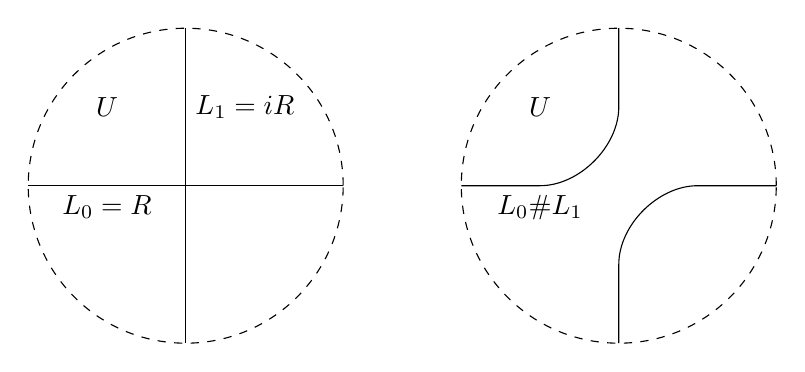
\begin{tikzpicture}
      \draw[dashed]  (0,0) circle[radius=2];
      \draw (-2,0) -- (2,0) (0,2) -- (0,-2);
      \node at (-1,1) {$U$};
      \node[right] at (0,1) {$L_1=i\mathbb R$};
      \node[below] at (-1,0) {$L_0=\mathbb R$};\begin{scope}[shift={(5.5,0)}]

      \draw[dashed]  (0,0) circle[radius=2];
      \node at (-1,1) {$U$};
      
      \node[below] at (-1,0) {$L_0\#L_1$};
      
      \draw (-2,0) .. controls (-1.5,0) and (-1.5,0) .. (-1,0) .. controls (-0.5,0) and (0,0.5) .. (0,1) .. controls (0,1.5) and (0,1.5) .. (0,2) ;
      \draw (2,0) .. controls (1.5,0) and (1.5,0) .. (1,0) .. controls (0.5,0) and (0,-0.5) .. (0,-1) .. controls (0,-1.5) and (0,-1.5) .. (0,-2);
\end{scope}
      
\end{tikzpicture}

%tag:000T
%label:"prp:polterovichSurgery"
%author:JeffHicks
%name:"Polterovich surgery of Lagrangian submanifolds"
%type:"proposition"
%source:"polterovich1991surgery"

 
Let $L_1, L_2\subset X$ be two Lagrangian submanifolds intersecting transversely at a single point $p$. 
Then there exists a Lagrangian submanifold $L_1\#_p L_2\subset X$ which
\begin{itemize}
        \item topologically is the connect sum of $L_1$ and $L_2$ at $p$. 
        \item Agrees with $L_1\cup L_2$ outside of a small neighborhood of $p$ in the sense that 
        \[L_1\#_p L_2|_{X\setminus U}=L_2\cup L_2|_{X\setminus U}.\]
\end{itemize}
 
%tag:000L
%label:"prf:polterovichSurgery"
%author:JeffHicks
%name:"construction of Polterovich surgery"
%type:"proof"
%parent:prp:polterovichSurgery

 
 

There exists a \snip{standard model}{lem:straightening} of two Lagrangian submanifold intersecting transversely at a point. Therefore, it suffices to construct a Lagrangian surgery neck for the standard intersection neighborhood $X=\CC^n$, $L_1=\RR^n$ and $L_2=\jmath\RR^n$.
We start by picking a \emph{surgery profile curve},  
\begin{align*}
      \gamma: [-R, R] \to& \CC\\
      t\mapsto& (a(t)+\jmath b(t))
\end{align*}
with the property that $a(t), b(t)$ are non-decreasing, and there exists a value $t_0$ so that 
\begin{itemize}
      \item  $\gamma(t)=t$ for $t< t_0$, and
      \item  $\gamma_\lambda(t)=\jmath t$ for $t>t_0$.
\end{itemize}
We denote the are bounded between the real axis, imaginary axis, and curve $\gamma$ by $\lambda$.
An example is drawn in \cref{fig:polterovichSurgeryProfile}.
%tag:000X
%label:"fig:polterovichSurgeryProfile"
%author:JeffHicks
%name:"surgery profile"
%type:"figure"
%parent:def:polterovichSurgery
%caption:"Surgery Profile for Polterovich surgery"



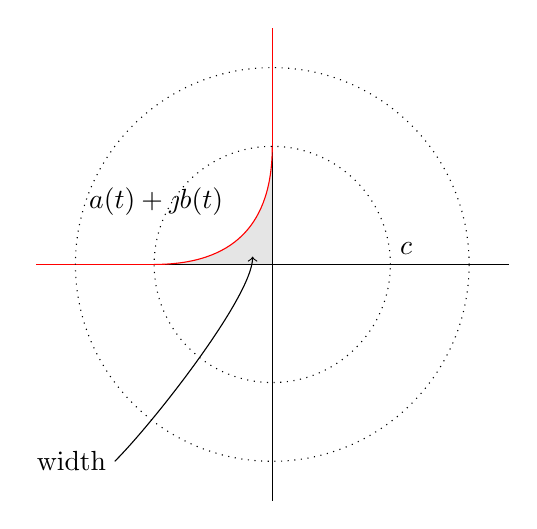
\begin{tikzpicture}

    \fill[fill=gray!20] (-1.5,0) .. controls (-0.5,0) and (-0.5,0) .. (0,0) .. controls (0,0.5) and (0,0.5) .. (0,1.5) .. controls (0,0.5) and (-0.5,0) .. (-1.5,0);
    
    \draw (0,3) -- (0,-3);
    \draw (3,0) -- (-3, 0);
    \draw[red] (-3, 0)--(-1.5,0) (0,1.5)--(0, 3);
    \draw[red] (-1.5,0) .. controls (-0.5,0) and (0,0.5) .. (0,1.5);
    \node[above left] at (-0.5,0.5) {$a(t)+\jmath b(t)$};
    \node[above right] at (1.5,0) {$c$};
    \draw[dotted]  (0,0) ellipse (1.5 and 1.5);
    \draw[dotted]  (0,0) ellipse (2.5 and 2.5);
    \draw[->] (-2,-2.5) .. controls (-1.5,-2) and (-0.25,-0.4) .. (-0.25,0.1);
    \node at (-2.55,-2.5) {width};
\end{tikzpicture}
This data provides a construction for the Lagrangian surgery neck:
\[
	L_1\#_\gamma L_2:=\left\{(\gamma(t)\cdot x_1,\ldots,  \gamma(t)\cdot x_n \text{ such that } x_i \in \RR^n,t\in \RR, \sum_{i} x_i^2=1\right\}.
\]
Note that when $t < t_0$ this parameterizes $(\RR\setminus B_r(0))\subset \CC^n$, and when $t > t_0$ the chart parameterizes $(\jmath \RR \setminus B_r(0))\subset \CC^n$. 
Therefore, this construction satisfies the condition that the surgery Lagrangian agrees with the surgery components outside of a small neighborhood of the surgery point.
This Lagrangian has the topology of $S^{n-1}\times \RR$, which is the local model for the connect sum $\RR^n\#_0\RR^n$.

It remains to show that the submanifold is Lagrangian \todo{}


\Cref{prp:polterovichSurgery} follows by taking $L_1\#_\gamma L_2$ for any suitable choice of $\gamma$.
 
Th surgery construction does not uniquely specify \emph{the} Lagrangian surgery of two Lagrangian submanifolds,  different choices of curves $\gamma$ produce different Lagrangian submanifolds.
Given a Lagrangian isotopy $\li_t: L\to C$ we associate \snip{flux cohomology class}{def:flux} $\Flux_{\li_t}\in H^1(L)$. 
We can similarly associate a flux class to a Lagrangian surgery.
A given surgery profile curve $\gamma$ can be extended to a family of Lagrangian surgery profiles by scaling the profile curve by a parameter $s$.  
This gives us a family of surgeries $L_1\#_{s\gamma} L_2$, which are Lagrangian isotopic.
The flux of the surgery is defined to be the flux of this isotopy. 
%label:"prp:fluxOfSurgery"
%author:JeffHicks
%name:"flux of Polterovich surgery"
%type:"proposition"

Let $L_0, L_1$ be two Lagrangian submanifolds which intersect transversely at a point, and let $U$ be a neighborhood of the point in which we implant a surgery neck. Suppose two profile curves $\gamma_0, \gamma_1$ have the same flux $\lambda$.
Then there exists a Hamiltonian supported on $U$ whose time one identifies $L_1\#_{\gamma_0} L_2$ and $L_1\#_{\gamma_1} L_2$.
The flux of $\gamma$ is the area bounded by $\gamma$ and the two axis. This is sometimes called the width or neck-width of the surgery.
We will write $L_1\#_{\lambda}L_2$ a Lagrangian connect sum determined by a surgery profile curve with flux $\lambda$.

The order of the summands plays an important role in Lagrangian surgery, as rarely are the Lagrangian $L_1\#L_2$ and $L_2\#L_1$ isotopic. 
%label:"exm:polterovichSurgery"
%author:JeffHicks
%name:"Polterovich surgery in $\RR^n$"
%type:"example"


We now visualize the Polterovich surgery for Lagrangian sections of $T^*\RR^n$.
The Lagrangians which we consider are two sections of the cotangent bundle. 
Let $L_1$ be the graph of $d(q_1^2+ \cdots+ q_n^2)$, and let $L_2$ be the graph of $d(-q_1^2-\cdots -q_n^2)$. 
In dimension 2, we can then draw $L_1\# L_2$ and $L_2\# L_1$ as multisections of the cotangent bundle. 
These multisections are sketched in \cref{fig:surgeryDim4}.
Note that one of surgeries creates a Lagrangian which has a ``neck'' visible in the projection to the base of the cotangent bundle.
The other surgery is generically a double-section of the cotangent bundle, except over the fiber of the intersection point where it is instead an $S^1$.


%label:"fig:surgeryDim4"
%author:JeffHicks
%name:"surgery of Lagrangians in $\dim(X)=2"
%type:"figure"
%parent:"con:dehnTwist"
%caption:"Lagrangian surgery of two sections of $T^*\RR^2$"


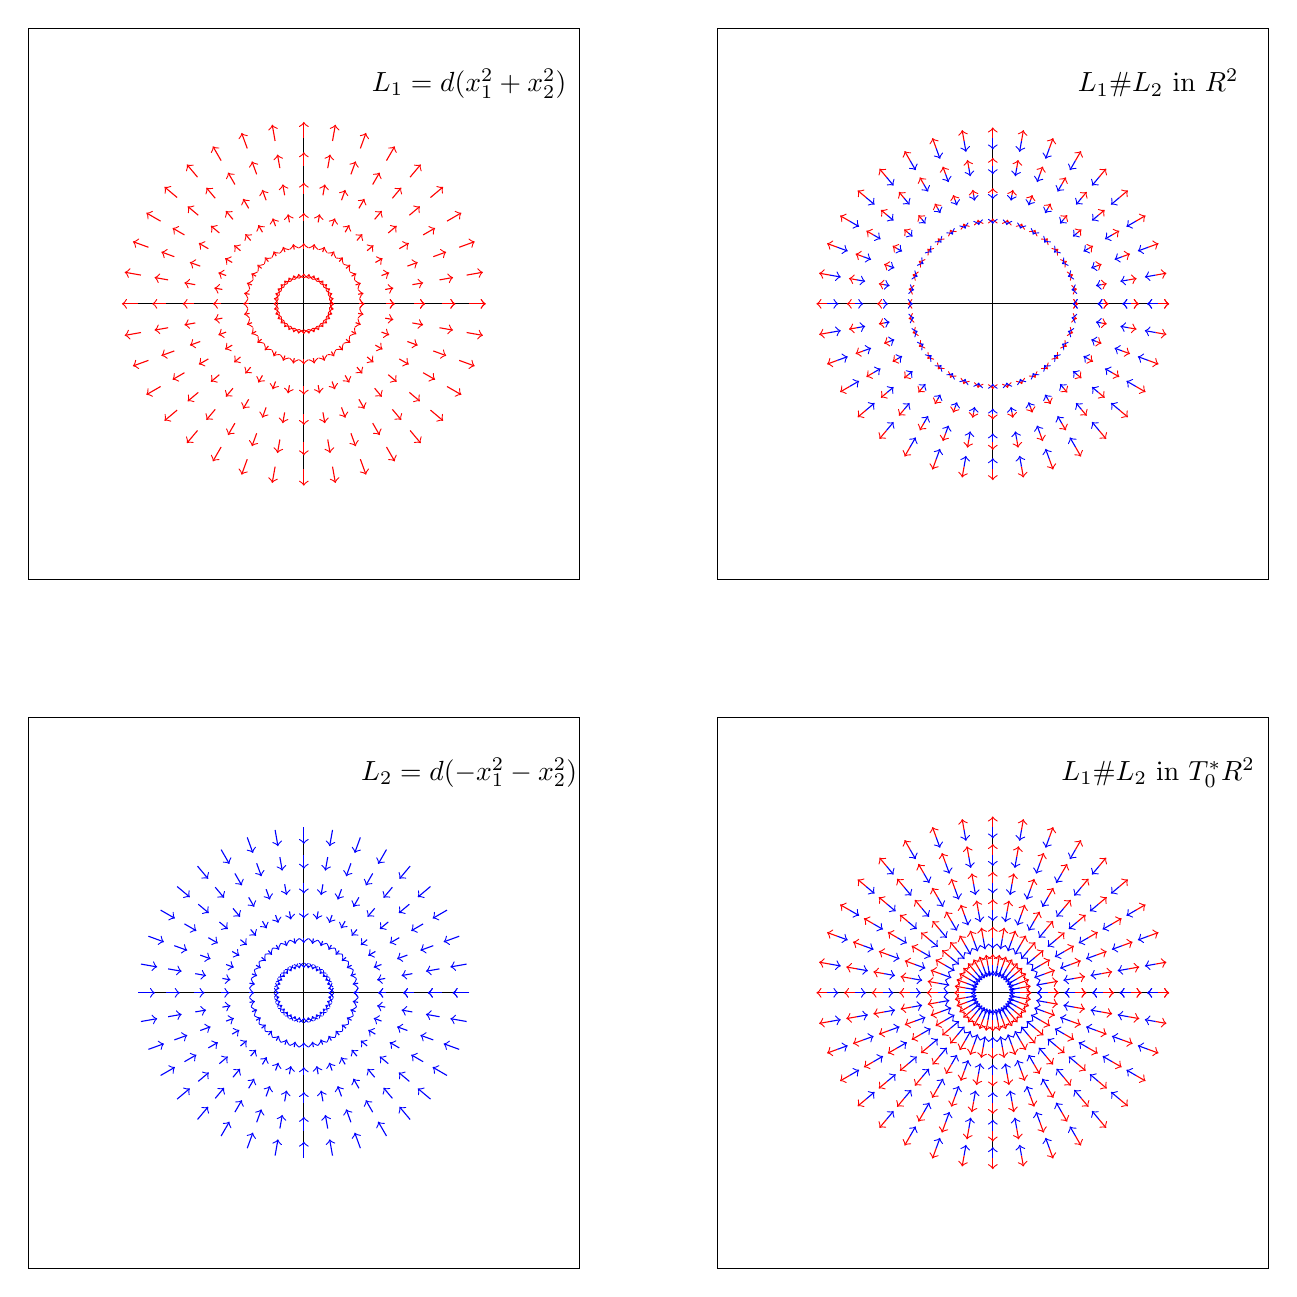
\begin{tikzpicture}[scale=.7]


    \begin{scope}[shift={(-12.5,1)}]
    \draw  (-5,5) rectangle (5,-5);
    \node at (3,4) {$L_1= d(x^2_1+x_2^2)$};
    
    \begin{scope}
    \draw (-3,0)--(3,0) (0,3)--(0,-3);
    \foreach \r in { .5, 1,1.5, 2,2.5, 3} {
        \foreach \t in {0,...,36} {
            \draw[->, red] ({\r * cos(10*\t)},{ \r * sin(10*\t) })-- ({1.1*\r * cos(10*\t)},{ 1.1*\r * sin(10*\t) });
            %\draw[->, blue] ({\r * cos(10*\t)},{ \r * sin(10*\t) })-- ({0.9*\r * cos(10*\t)},{ 0.9*\r * sin(10*\t) });
        }
    }
    \end{scope}
    \end{scope}
    
    
    \begin{scope}[shift={(-12.5,-11.5)}]
    
    
    \draw  (-5,5) rectangle (5,-5);
    
    \node at (3,4) {$L_2=d(-x^2_1-x_2^2)$};
        \begin{scope}
    \draw (-3,0)--(3,0) (0,3)--(0,-3);
    \foreach \r in { .5, 1,1.5, 2,2.5, 3} {
        \foreach \t in {0,...,36} {
            %\draw[->, red] ({\r * cos(10*\t)},{ \r * sin(10*\t) })-- ({1.1*\r * cos(10*\t)},{ 1.1*\r * sin(10*\t) });
            \draw[->, blue] ({\r * cos(10*\t)},{ \r * sin(10*\t) })-- ({0.9*\r * cos(10*\t)},{ 0.9*\r * sin(10*\t) });
        }
    }
    \end{scope}
    \end{scope}
    
    \begin{scope}[]
    
    \begin{scope}[shift={(0,1)}]
    
    
    \draw  (-5,5) rectangle (5,-5);
    
    \node at (3,4) {$L_1\#L_2$ in $\mathbb R^2$};
    
    
    
    \begin{scope}
    \draw (-3,0)--(3,0) (0,3)--(0,-3);
    \foreach \r in { .5, 1,1.5, 2} {
        \foreach \t in {0,...,36} {
            \draw[->, red] ({(\r+1) * cos(10*\t)},{ (\r+1) * sin(10*\t) })-- ({(1.1*\r +1)* cos(10*\t)},{ (1.1*\r+1) * sin(10*\t) });
            \draw[->, blue] ({(\r+1) * cos(10*\t)},{ (\r+1) * sin(10*\t) })-- ({(0.9*\r+1) * cos(10*\t)},{( 0.9*\r +1)* sin(10*\t) });
        }
    }
    \end{scope}
    \end{scope}
    \begin{scope}[shift={(0,-11.5)}]
    
    
    \draw  (-5,5) rectangle (5,-5);
    
    \node at (3,4) {$L_1\#L_2$ in $T^*_0\mathbb R^2$};
    
    \begin{scope}
    \draw (-3,0)--(3,0) (0,3)--(0,-3);
    \foreach \r in {.5, 1,1.5, 2,2.5, 3} {
        \foreach \t in {0,...,36} {
            \draw[->, red] ({\r * cos(10*\t)},{ \r * sin(10*\t) })-- ({(\r+.2) * cos(10*\t)},{ (\r+.2) * sin(10*\t) });
            \draw[->, blue] ({\r * cos(10*\t)},{ \r * sin(10*\t) })-- ({(\r-.2) * cos(10*\t)},{ (\r-.2) * sin(10*\t) });
        }
    }
    \end{scope}
    \end{scope}
    
    \end{scope}
    
    \end{tikzpicture}


 

